\documentclass[uplatex]{jsarticle}
\usepackage[utf8]{inputenc}

% 文字コード関連の設定
\usepackage{otf}
% 箇条書きのパラメータ関連の設定
\usepackage{paralist}
% ソースコード関連の設定
\usepackage{listings,jlisting}
% プログラムのソースコード
\lstdefinestyle{program}{
    basicstyle={\small\ttfamily},
    breaklines=true,
    columns=fixed,
    basewidth=0.5em,
    % スペースを可視化するかどうか
    showstringspaces=false,
    % 枠線 trbl(大文字で二重線)
    frame={tb},
    % フレームと本文の間のマージン
    framesep=8pt,
    % 行番号
    numbers=left,
    numbersep=2zw,
    % フォントサイズ
    numberstyle={\scriptsize},
    % マージン
    xrightmargin=0zw,
    xleftmargin=3zw,
    % 行間
    lineskip=-0.2ex,
    % タブ数
    tabsize=4,
    % キャプション名の場所
    captionpos=t,
}
% プログラムの一部
\lstdefinestyle{code}{
    basicstyle={\small\ttfamily},
    breaklines=true,
    columns=fixed,
    basewidth=0.5em,
    % スペースを可視化するかどうか
    showstringspaces=false,
    % フレームと本文の間のマージン
    framesep=8pt,
    % マージン
    xrightmargin=0zw,
    xleftmargin=2.5zw,
    % 行間
    lineskip=-0.2ex,
    % タブ数
    tabsize=4,
}
% コマンド
% 角が丸いフレーム付き(文字サイズsmall)
\lstdefinestyle{command}{
    basicstyle={\small\ttfamily},
    breaklines=true,
    columns=fixed,
    basewidth=0.5em,
    showstringspaces=false,
    frame={trbl},
    frameround={tttt},
    framesep=8pt,
    framerule=0pt,
    xrightmargin=1zw,
    xleftmargin=1zw,
    lineskip=-0.2ex,
    tabsize=4,
}
% 角が丸いフレーム付き
\lstdefinestyle{withframe}{
    basicstyle={\ttfamily},
    breaklines=true,
    columns=fixed,
    basewidth=0.5em,
    showstringspaces=false,
    frame={trbl},
    frameround={tttt},
    framesep=8pt,
    framerule=0pt,
    xrightmargin=1zw,
    xleftmargin=1zw,
    lineskip=-0.5ex,
    tabsize=4,
}
% キャプション名
\renewcommand{\lstlistingname}{プログラム}
% 囲い関連の設定
\usepackage{ascmac}
% マージンの設定
\usepackage[left=30mm,right=30mm,top=30mm,bottom=30mm]{geometry}
\renewcommand{\baselinestretch}{1.15}
% 画像関連
\usepackage[dvipdfmx]{graphicx}
% フォント
\usepackage{newtxtext,newtxmath}
% URL
\usepackage{url}
% 目次
\usepackage[dvipdfmx]{hyperref}
\usepackage{pxjahyper}
\hypersetup{
    setpagesize=false,
    bookmarksnumbered=true,
    bookmarksopen=true,
    colorlinks=true,
    linkcolor=black,
    citecolor=black,
    urlcolor=black,
}


\begin{document}
\title{Windows Subsystem for Linux(WSL)\\とWindows Terminalの導入}
\author{濵田 幸希}
\date{2020年11月7日}
\maketitle

\tableofcontents

\newpage
\section{WSLの導入}
\subsection{Linux 用 Windows サブシステムを有効にする}
管理者権限でPowerShellを起動し,以下のコマンドを実行する.
その後,PCを再起動する.
\vspace{5pt}

\begin{lstlisting}[style=command]
$ dism.exe /online /enable-feature 
  /featurename:Microsoft-Windows-Subsystem-Linux /all /norestart
\end{lstlisting}


\begin{figure}[h]
\centering
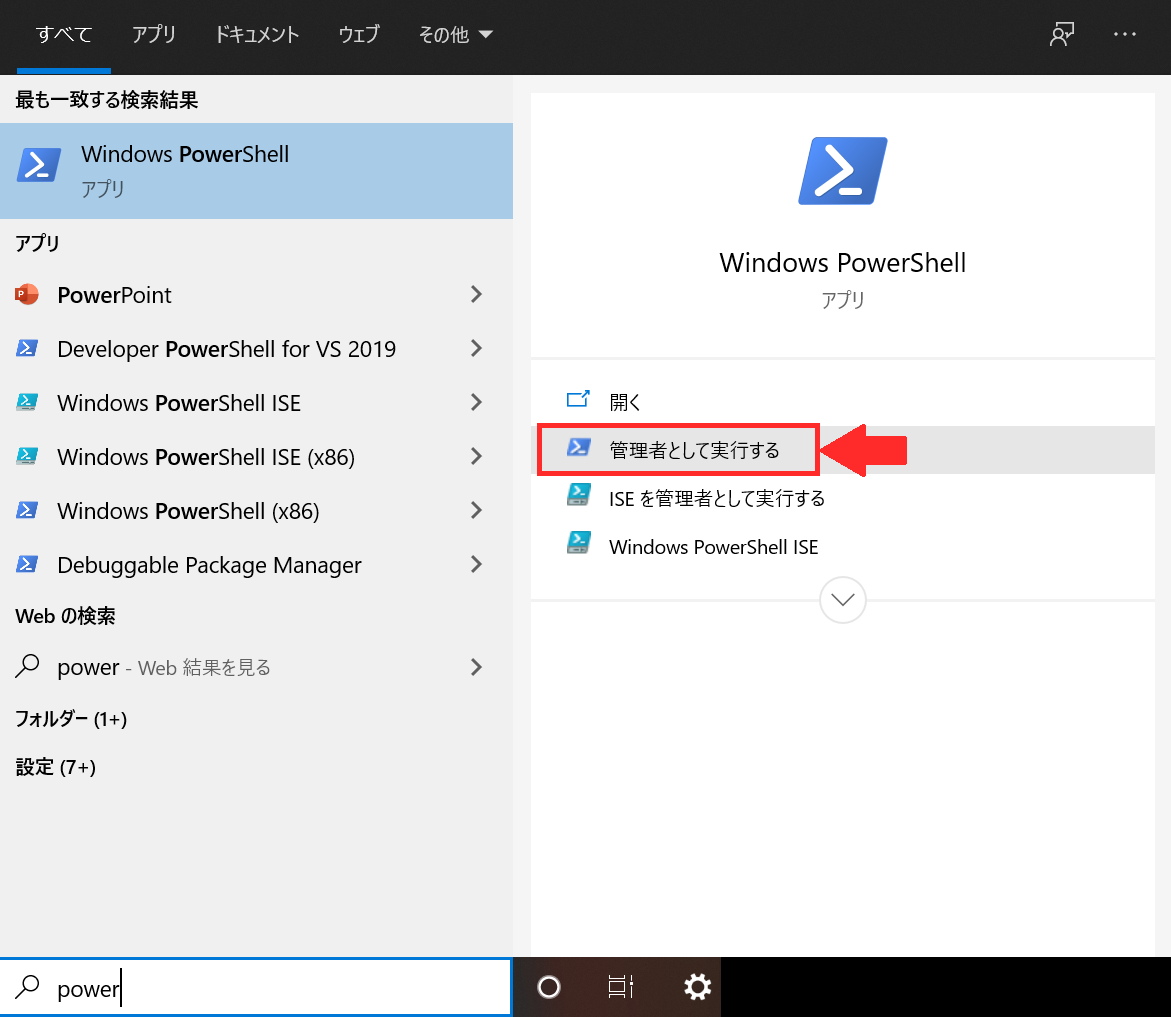
\includegraphics[scale=0.5]{./図/powershell.png}
\caption{PowerShellを管理者権限で起動}
\label{fig:powershell}
\end{figure}

\subsection{WSL2を導入したい場合}
WSLをさらに高性能化させたWSL2を使いたい場合は,
\begin{center}
\url{https://docs.microsoft.com/ja-jp/windows/wsl/install-win10}
\end{center}
\noindent
にしたがえば,導入することができる.
しかし,Hyper-Vを有効化することでVirtualBoxなどの仮想化ソフトウェアが使用できなくなったり
\footnote{VMware Workstation 15.5.5以降ではHyper-Vとの共存が可能になった(Windows 10 May 2020 Updateを適用しているPCのみ対応している).}
,WSL2のプロセスVmmemのメモリ使用量が増加し続けたり
\footnote{\url{https://qiita.com/yoichiwo7/items/e3e13b6fe2f32c4c6120}}
などといった問題がある.

\subsection{Linux ディストリビューションをインストールする}
Microsoft Storeを起動し,「Ubuntu」と検索する.
その後,必要なLinux ディストリビューションをインストールする(ここでは一番左のUbuntuを選択).
インストールに関係ないところで選択肢が出てきたら,全部無視でかまわない.

\begin{figure}[h]
\centering
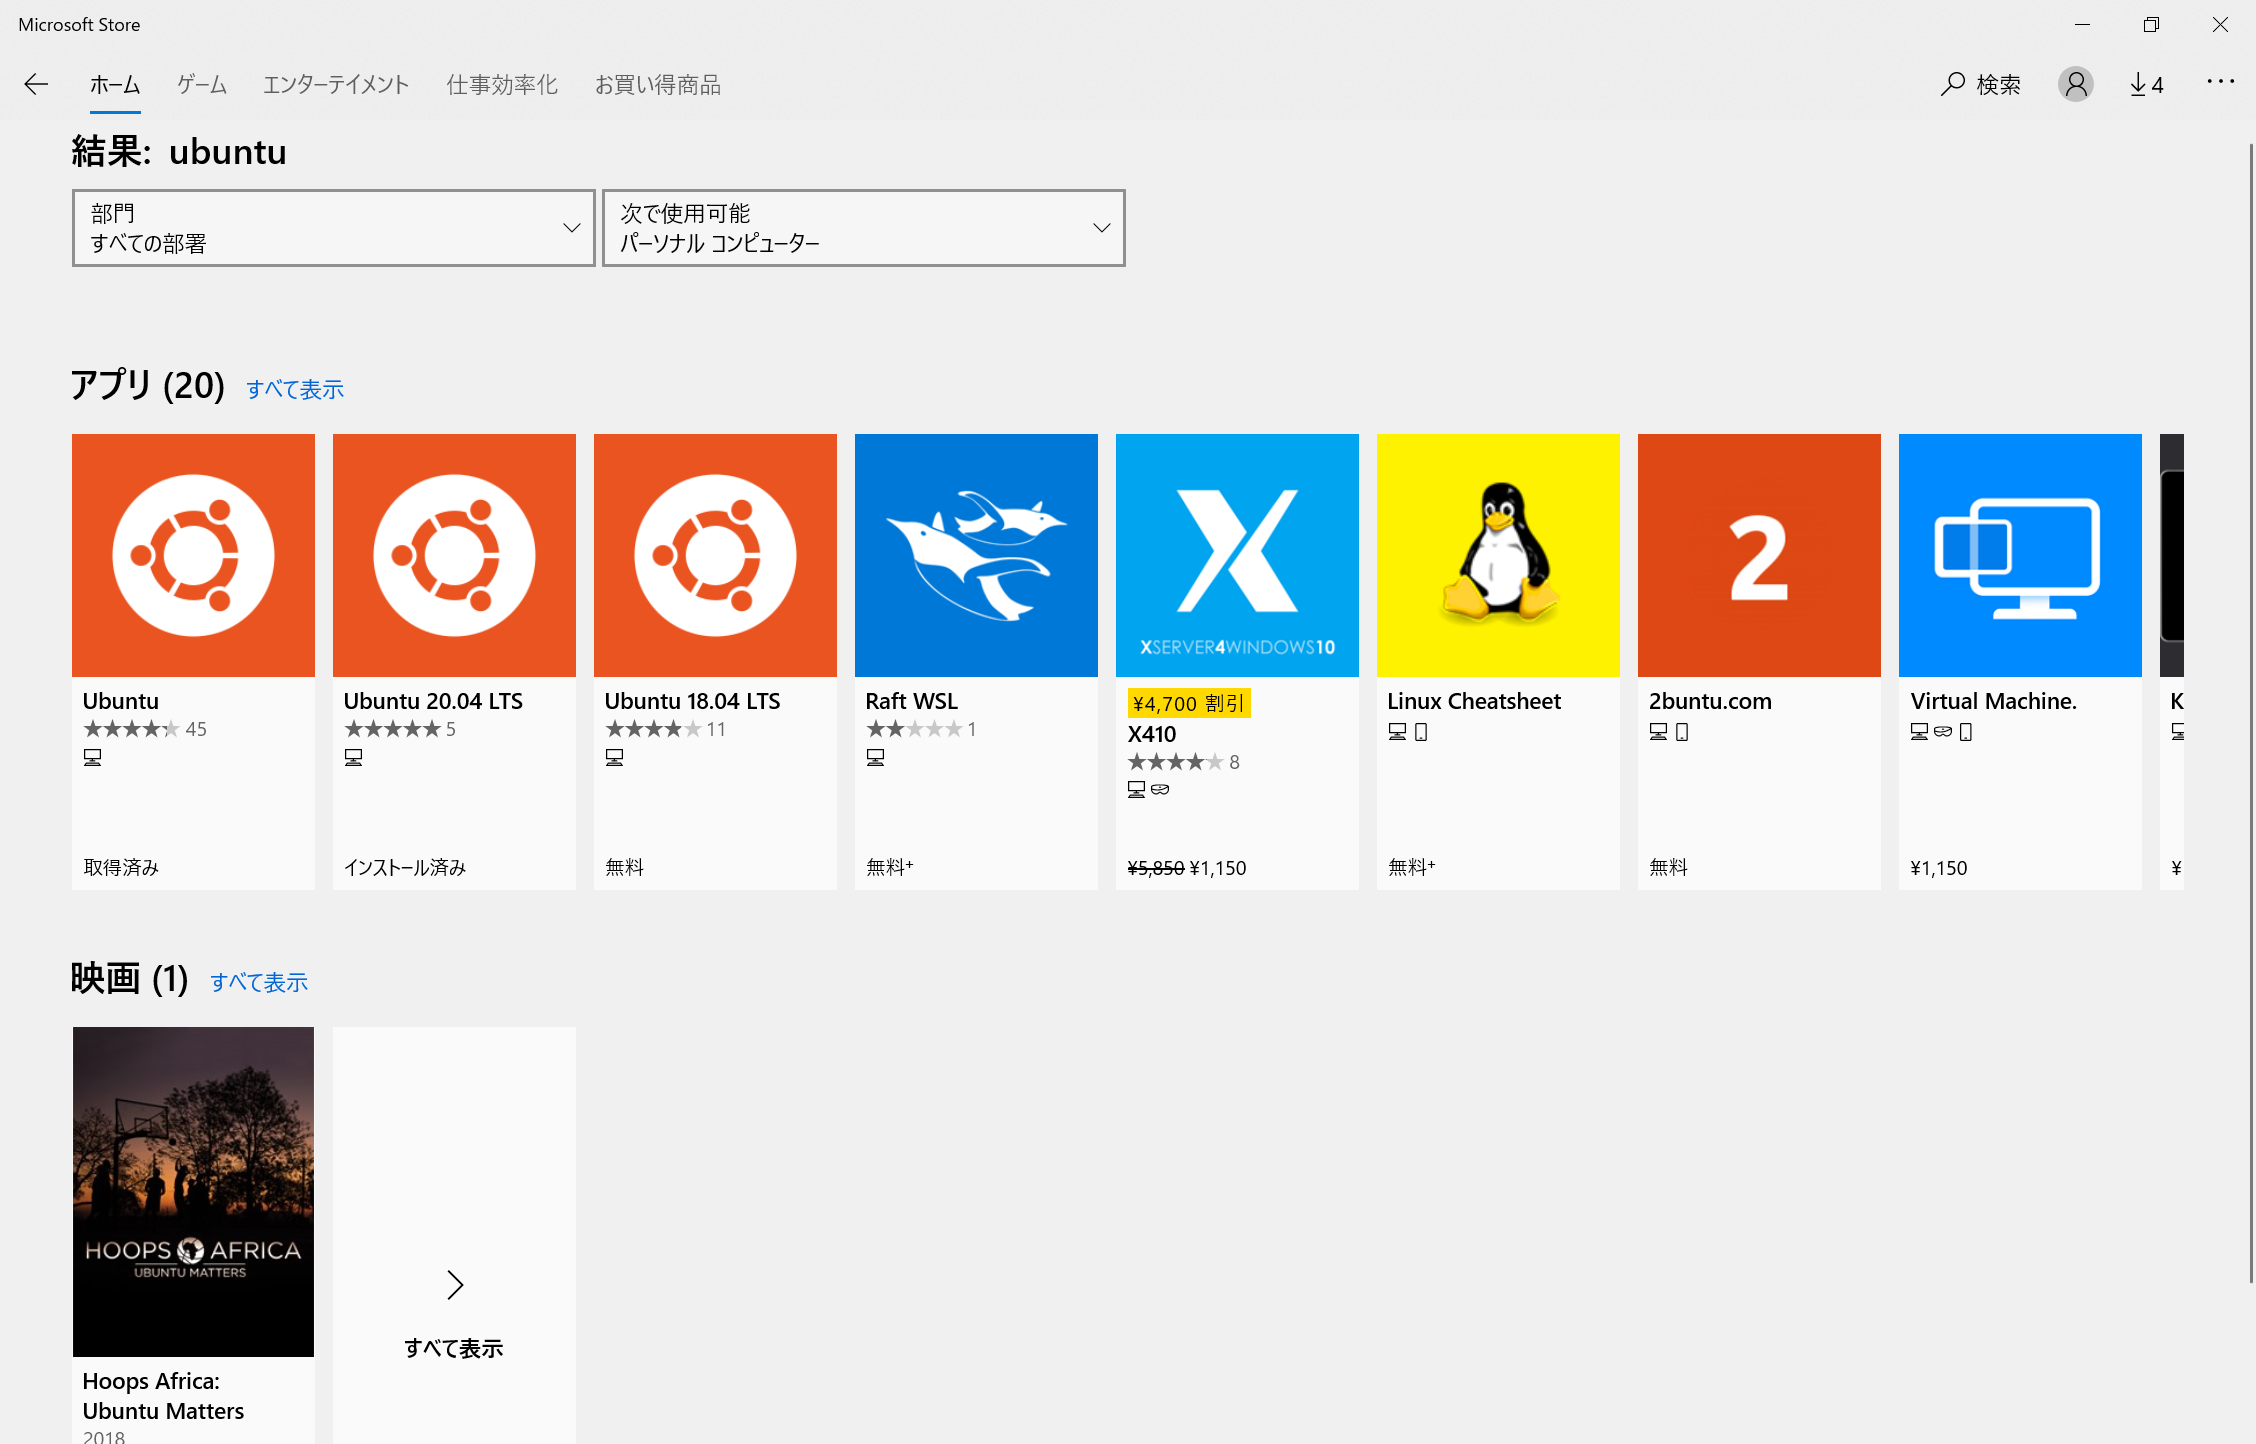
\includegraphics[scale=0.25]{./図/search_ubuntu.png}
\caption{Microsoft Storeで「Ubuntu」と検索}
\end{figure}

\subsection{初期設定}
インストールができたら,起動して初期設定を行う.好きなユーザ名(英語)とパスワード(高頻度で打つので,複雑にしすぎると後が大変)を入力し,Enterを押して進める.

\begin{figure}[h]
\centering
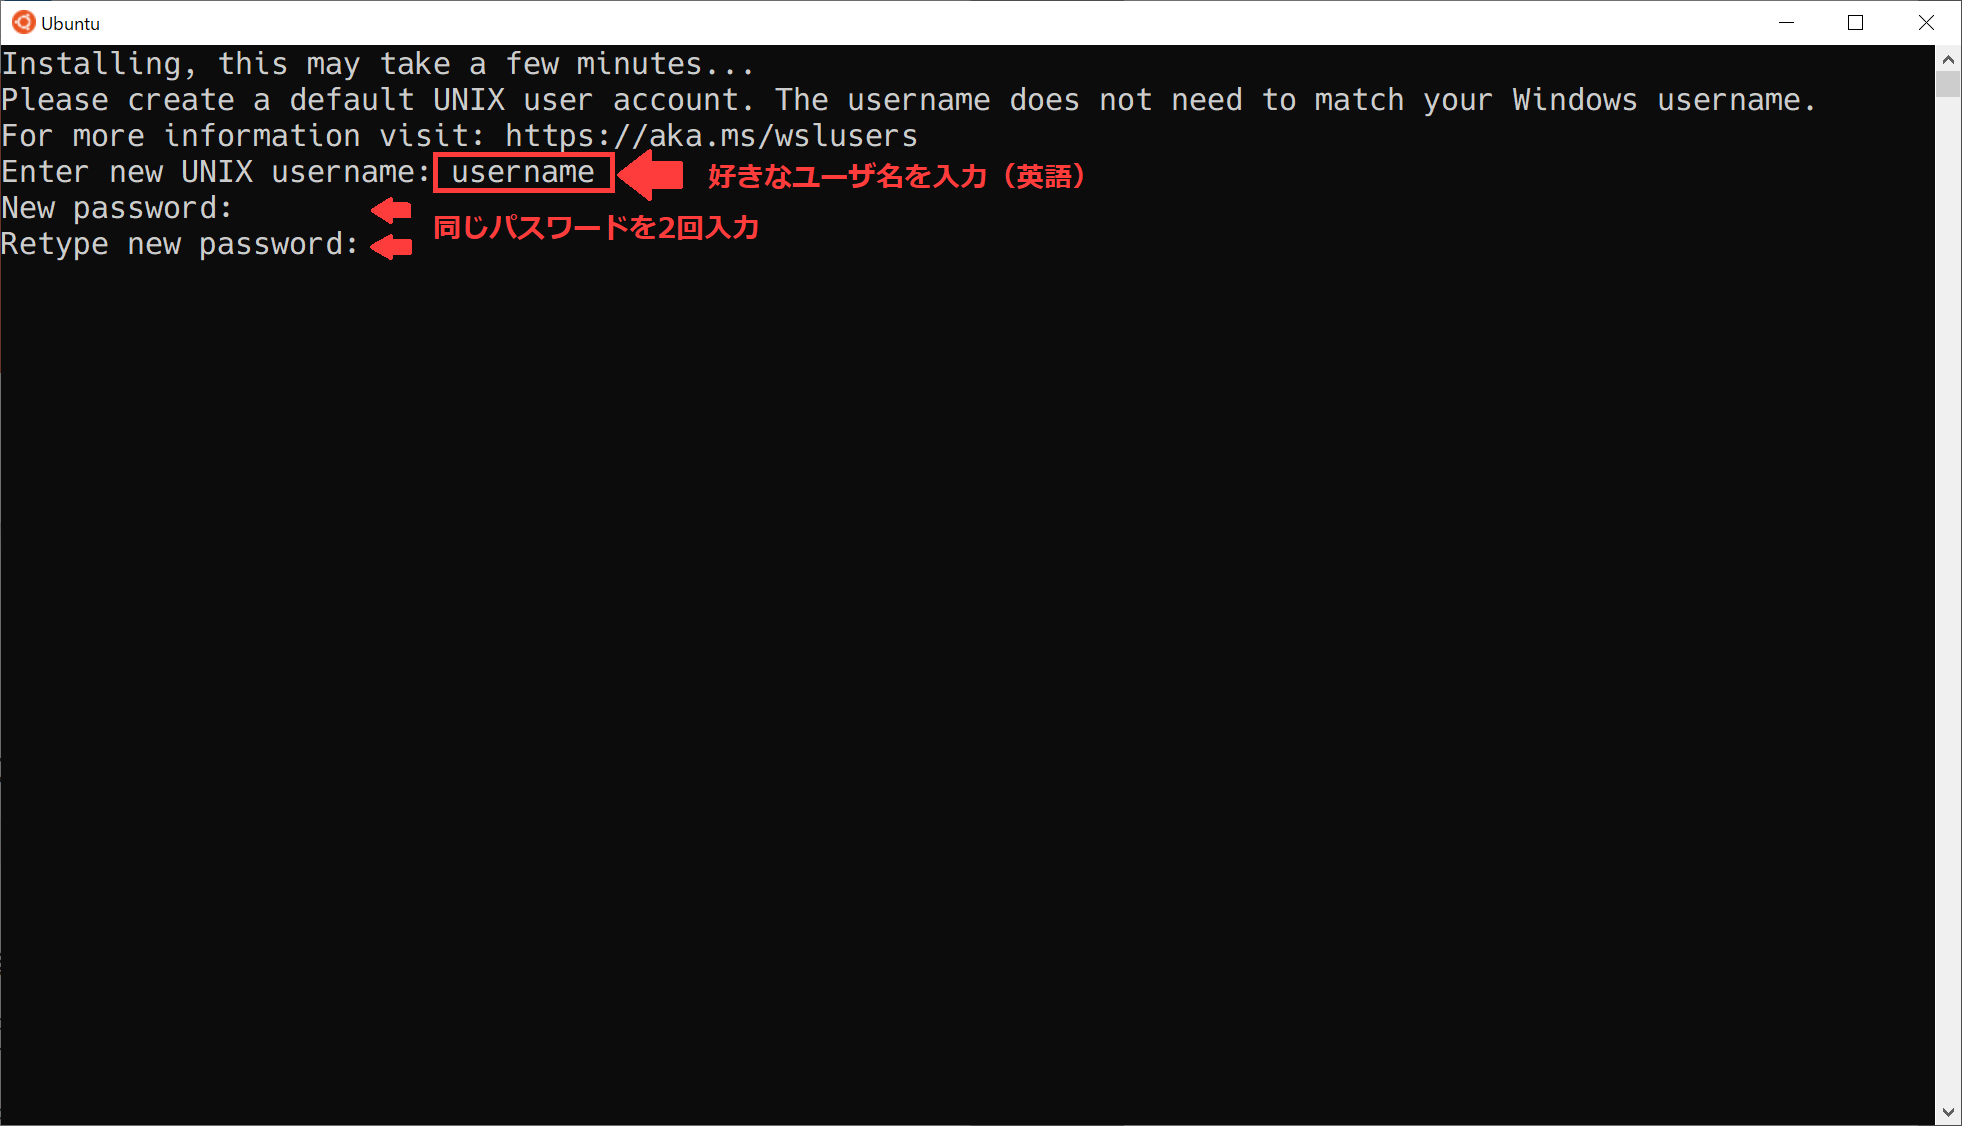
\includegraphics[scale=0.4]{./図/start_ubuntu.png}
\caption{Ubuntuの初期設定}
\end{figure}

\newpage
\subsection{初期設定に失敗した場合}
初期設定に失敗するとユーザが作られず,図\ref{fig:root}のようにデフォルトがrootユーザになってしまう.
このままだと権限周りで様々な問題が発生してしまうので,再インストールかユーザの作成が必要となる.

\begin{figure}[h]
\centering
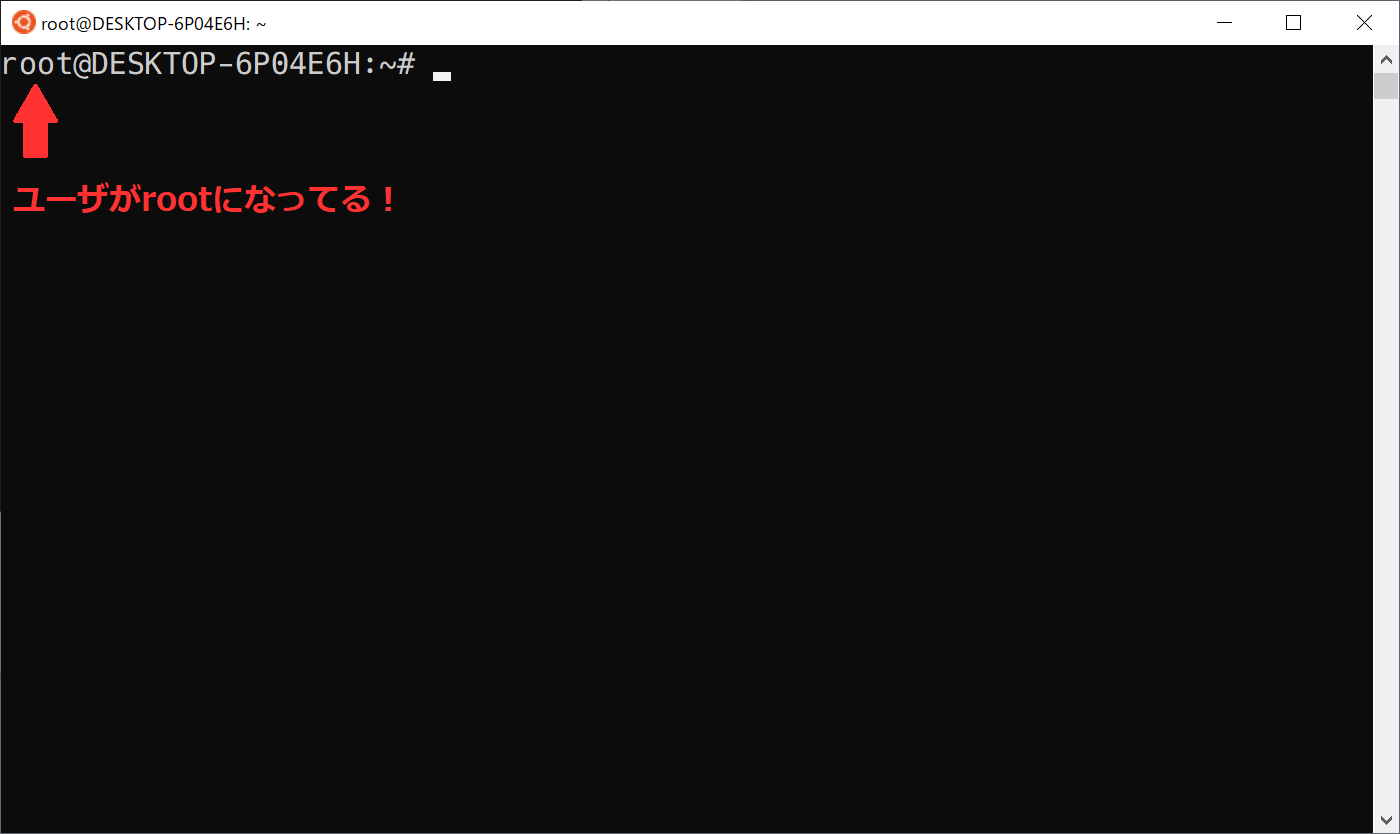
\includegraphics[scale=0.45]{./図/root.png}
\caption{デフォルトがrootユーザ}
\label{fig:root}
\end{figure}

\subsection{Ubuntuの再インストール方法}
スタートから「Ubuntu」と検索し,アンインストールをクリックして進める.
その後,Microsoft Storeからもう一度インストールをする.

\begin{figure}[h]
\centering
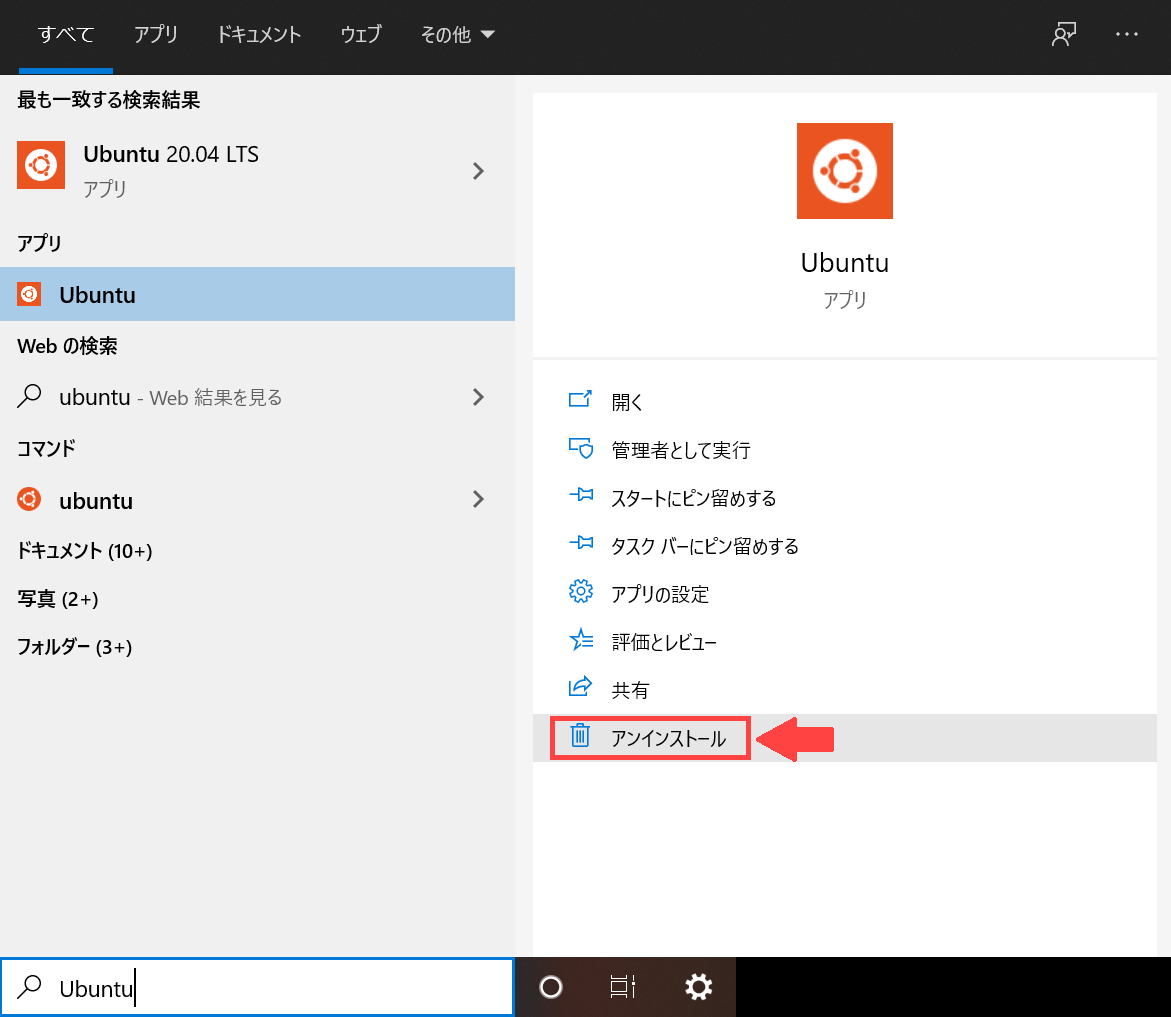
\includegraphics[scale=0.45]{./図/uninstall.png}
\caption{Ubuntuのアンインストール}
\end{figure}

\newpage

\section{Windows Terminalの導入}
\subsection{Windows Terminalのインストール}
Microsoft StoreからWindows Terminalをインストールする(Previewではない方を選ぶ).

\begin{figure}[h]
\centering
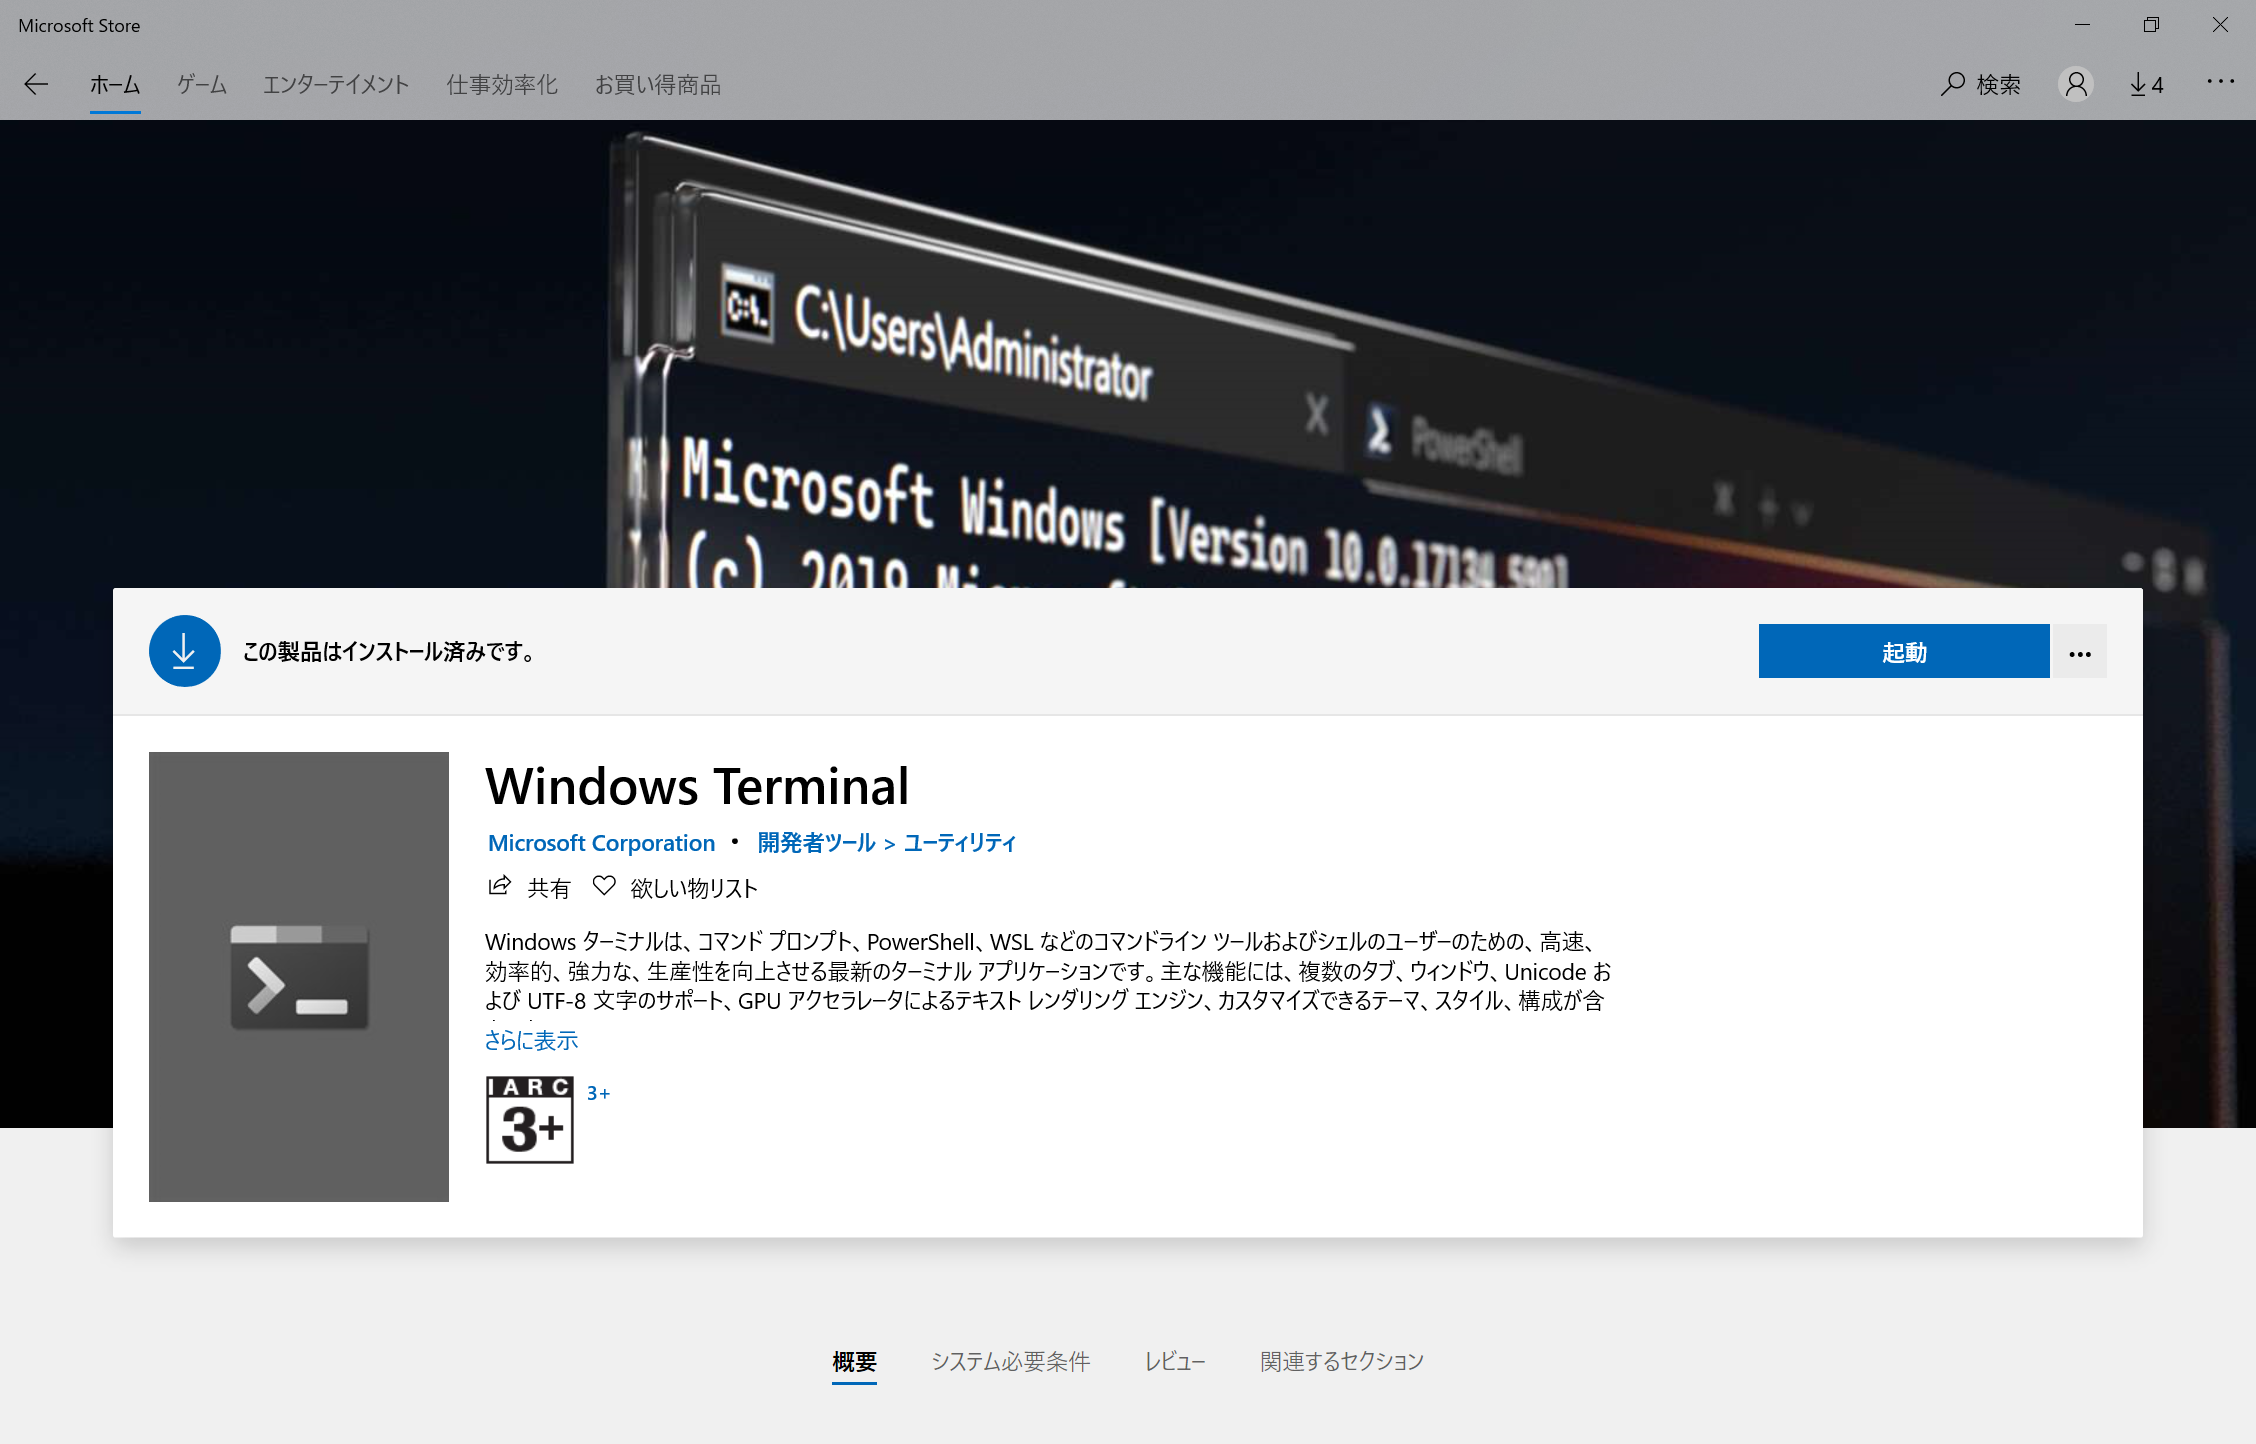
\includegraphics[scale=0.3]{./図/install_terminal.png}
\caption{Windows Terminalのインストール}
\end{figure}

Windows Terminalを起動すると,初期設定ではPowerShellが開かれる.

\begin{figure}[h]
\centering
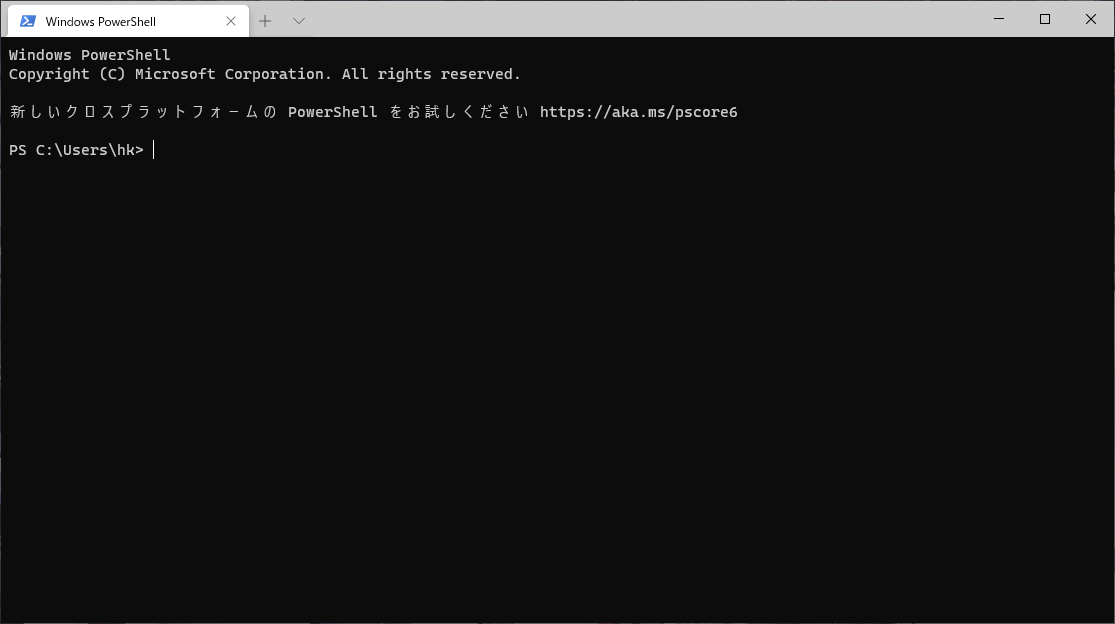
\includegraphics[scale=0.4]{./図/startup_terminal.png}
\caption{Windows Terminalの初期画面}
\end{figure}

\newpage
\subsection{基本的な設定}
\verb|ctrl|と\verb|,|を押すと,Windows Terminalの設定ファイルsettings.jsonがデフォルトのテキストエディタで開かれる.
まず,デフォルトでUbuntuが開かれるように設定する.
\$schemaの次の行にあるdefaultProfileの内容を以下のように書き換える.
\vspace{5pt}
\begin{lstlisting}[style=code]
    "defaultProfile": "{2c4de342-38b7-51cf-b940-2309a097f518}"
\end{lstlisting}

書き換える値はprofilesのlistの中にある各プロファイルのguidを参照すればよい.
\vspace{5pt}
\begin{lstlisting}[style=code]
           {
                "guid": "{2c4de342-38b7-51cf-b940-2309a097f518}",
                "hidden": false,
                "name": "Ubuntu",
                "source": "Windows.Terminal.Wsl",
            },
\end{lstlisting}

次に,profilesのdefaultの中にフォント関連の設定を記述する
\footnote{フォントは\url{https://github.com/miiton/Cica}がおすすめ.}.
\vspace{5pt}
\begin{lstlisting}[style=code]
    "profiles": {
        "defaults": {
            // Put settings here that you want to apply to all profiles.
            // フォント名
            "fontFace": "Cica",
            // フォントサイズ
            "fontSize": 13,
        },
\end{lstlisting}

初期設定ではWindows10のホームディレクトリから始まるので,
Ubuntuのホームディレクトリから始まるように,Ubuntuのプロファイル内に以下の内容を追記する.

\vspace{5pt}
\begin{lstlisting}[style=code]
            {
                "guid": "{2c4de342-38b7-51cf-b940-2309a097f518}",
                "hidden": false,
                "name": "Ubuntu",
                "source": "Windows.Terminal.Wsl",
                // 追記
                "startingDirectory": "//wsl$/Ubuntu/home/(設定したユーザ名)",
            },
\end{lstlisting}

\newpage
\subsection{テーマの設定}
テーマはsettings.jsonのschemesの中に記述することで作成できる.
1から自作することもできるが,\url{https://windowsterminalthemes.dev/}で様々な種類のテーマが配布されている.
ここから好きなものを選んでGet themeを左クリックするとコピーされるので,schemesの中に貼り付ける.
\vspace{5pt}
\begin{lstlisting}[style=code]
    "schemes": [
        {
            "name": "Argonaut",
            "black": "#232323",
            "red": "#ff000f",
            "green": "#8ce10b",
            "yellow": "#ffb900",
            "blue": "#008df8",
            "purple": "#6d43a6",
            "cyan": "#00d8eb",
            "white": "#ffffff",
            "brightBlack": "#444444",
            "brightRed": "#ff2740",
            "brightGreen": "#abe15b",
            "brightYellow": "#ffd242",
            "brightBlue": "#0092ff",
            "brightPurple": "#9a5feb",
            "brightCyan": "#67fff0",
            "brightWhite": "#ffffff",
            "background": "#0e1019",
            "foreground": "#fffaf4"
        },
    ],
\end{lstlisting}

作成したテーマをUbuntuで適用するためには,Ubuntuのプロファイル内に以下の内容を追記する.

\vspace{5pt}
\begin{lstlisting}[style=code]
            {
                "guid": "{2c4de342-38b7-51cf-b940-2309a097f518}",
                "hidden": false,
                "name": "Ubuntu",
                "source": "Windows.Terminal.Wsl",
                "startingDirectory": "//wsl$/Ubuntu/home/(設定したユーザ名)",
                // 追記
                "colorScheme": "Argonaut",
            },
\end{lstlisting}

\newpage
\subsection{詳しい設定方法について}
\url{https://docs.microsoft.com/ja-jp/windows/terminal/}を参照.

\begin{figure}[h]
\centering
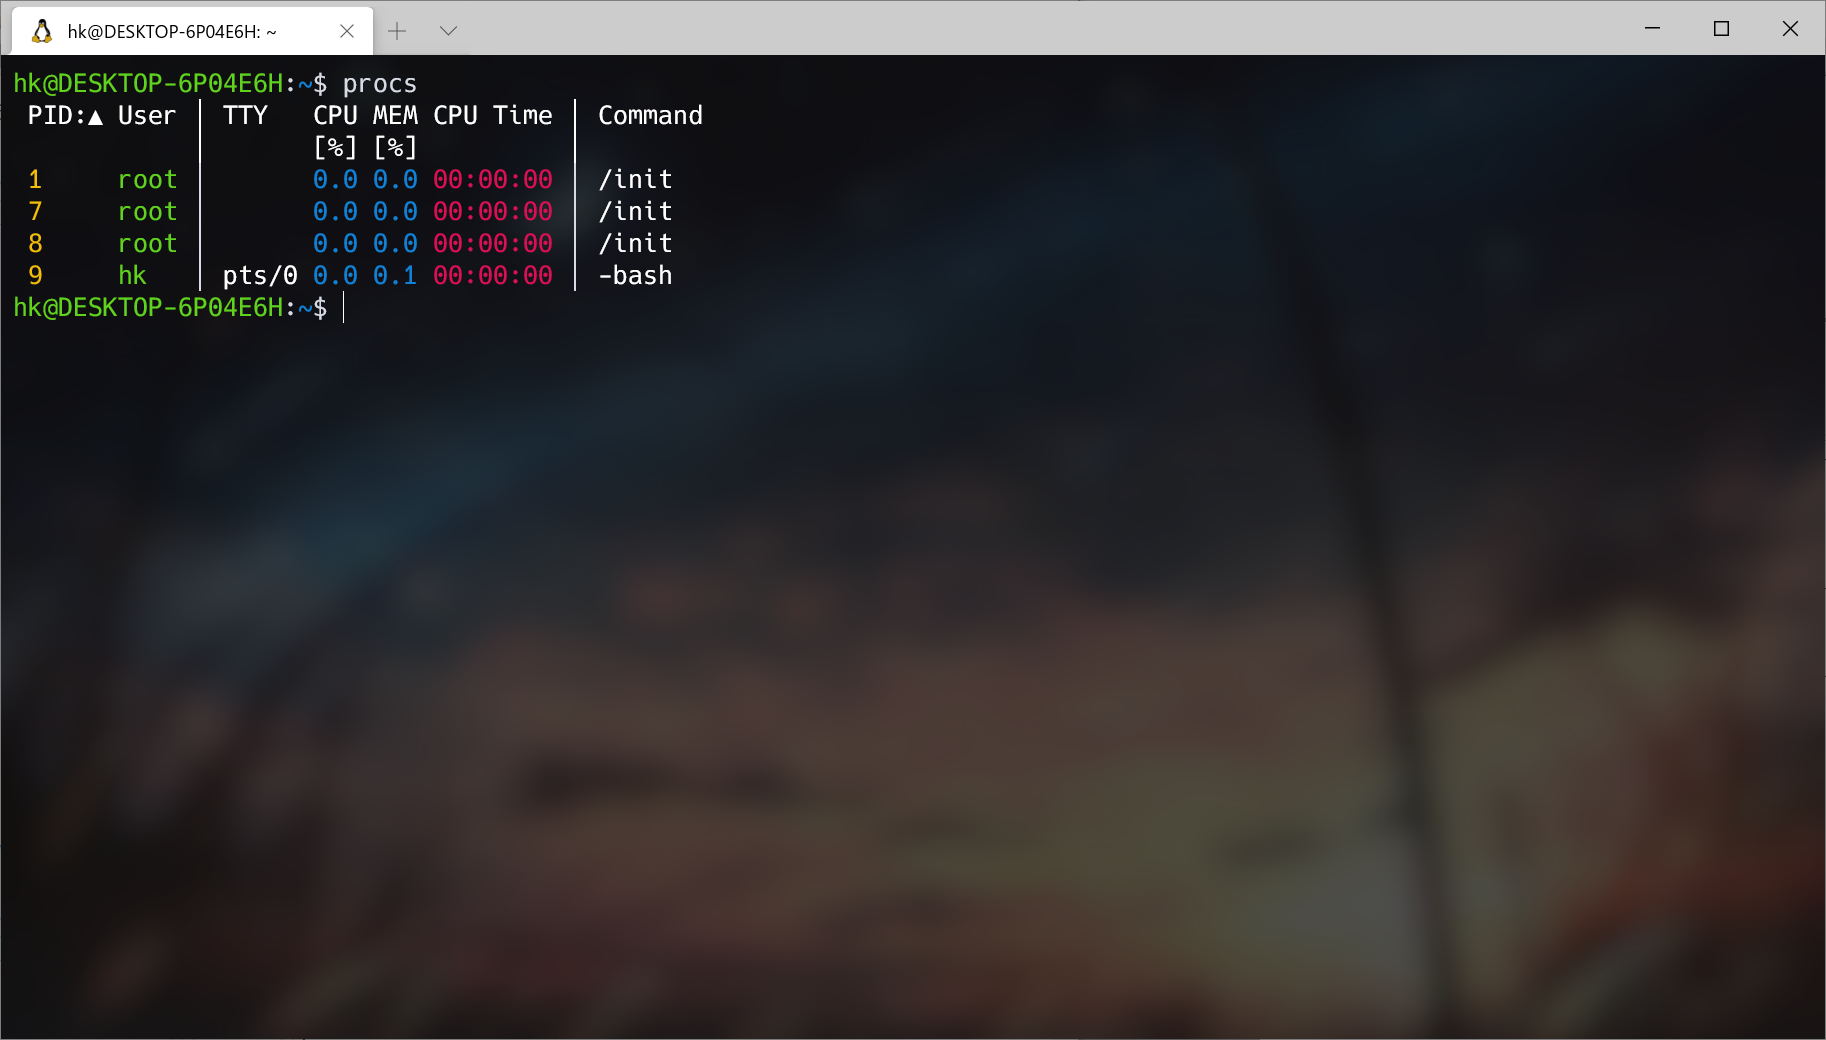
\includegraphics[scale=0.45]{./図/myterminal.png}
\caption{Windows Terminalのカスタマイズ例}
\end{figure}

\newpage
\section{Ubuntuを入れた後に最低限やるべきこと}
\subsection{アップデートとアップグレード}
最初にアップデートとアップグレードを行う.選択肢が出たら,yを押して続行する.

\vspace{5pt}
\begin{lstlisting}[style=command]
$ sudo apt update
$ sudo apt upgrade
\end{lstlisting}

\subsection{ディレクトリの色修正}
WSLでlsをすると,ディレクトリに背景色が付いていて見にくいので,それを修正する.
手順は
\url{https://qiita.com/Yumaski/items/53fbd1684bee303d65aa}
を参照.
\verb|.zshrc|のところは\verb|.bashrc|に置き換えて読むこと.


\subsection{build essentialのインストール}
CやC++などのプログラムをコンパイルするために必要なソフトウェアをインストールする.

\vspace{5pt}
\begin{lstlisting}[style=command]
$ sudo apt install build-essential
\end{lstlisting}

\end{document}
